%In this section, we present our study results by answering our research questions. For each question, we discuss the motivation behind it, the approach to answering it and finally the results obtained. 
%\\
%
%\noindent\textbf{RQ1:} \textbf{How much do logs change over time and why do the changes occur?}
%\\

%\noindent\textbf{Motivation}

%Research has shown that logs evolve along with the code~\cite{IanContextinformation}. When logs are changed, the log  processing tools which are dependent on them also have to get updated. This results in costly maintenance effort. To understand the cost, we have to understand how frequent changes to logs are. Hence, we explore the frequency of changes to logs in our studied systems and why they are changed.\\

%\noindent \textbf{Approach}


%\begin{table*}
%	\centering
%	\caption{Distribution of log changes in different projects}
%	\label{tba:logchangeDistribution}
%	\begin{tabular}{l|>{\centering}p{.1\columnwidth}>{\centering}p{.01\columnwidth} 
%			p{0.01\columnwidth} }
%		\cline{1-4}  	\multicolumn{1}{|c}{Projects}    & \multicolumn{1}{|c}{Never Changed (\%) }  &  \multicolumn{1}{|c}{Changed (\%) }	   &  \multicolumn{1}{|c}{Frequently Changed (\%) }\\ \cline{1-4}   
%		
%		Life Ray      & 78.67     & 19.66 & 1.66           \\
%		
%		Camel      & 55.43    & 37.32 & 7.25            \\
%		ActiveMq   & 34.78     & 62.02 & 3.20           \\
%		CloudStack & 19.68     & 68.61 & 11.71          \\ \cline{1-4}
%	\end{tabular}
%\end{table*}

%\begin{table*}
%	\centering
%	\caption{Distribution of log changes in different projects}
%	\label{tba:logtype}
%	\begin{tabular}{l|llll}
%		\cline{1-5}  	\multicolumn{1}{|c}{Projects}    & \multicolumn{1}{|c}{ ActiveMQ }  &  \multicolumn{1}{|c}{ Camel}	   &  \multicolumn{1}{|c}{ Cloudstack }  & 
%		\multicolumn{1}{|c|}{ Liferay } \\ \cline{1-5}   
%		
%		Log relocation (\%)       & 20.05     & 20.80 &  53.32  & 49.42         \\
%		
%		Log text change (\%)      & 26.59    & 26.37 & 15.54    & 32.70       \\
%		Log variable change (\%)   & 53.18     & 52.75 & 31.08 &  16.75     \\
%		Change of log level (\%) & 0.18   & 0.08 & 0.04  &  1.13       \\ 
%%		Text and variable change (\%) & 2.33     & 6.39 & 22.0   &  30.59    \\ 
%\cline{1-5}
%	\end{tabular}
%\end{table*}


In this paper we aim to get a better understanding of the
unstable logs in an application so that we can improve the maintenance of log processing tools. In this section we present our rationale for selecting the applications we studied and present the results of our preliminary analysis in the four studied applications.

\subsection{Subject systems}
We evaluate our approach through a case study on four open source applications. We select these projects on the following two criteria:
\begin{itemize}
	\item \textbf{Log usage -} We select applications that make use of extensive logging in their source code. 
	%	This helps to improve the performace of the random forest classifier and to identify the factors which effect log stability.
	\item \textbf{Project activity -} We pick applications which have a large user base and commit history.
	\item \textbf{Programming language -} We pick applications written in Java as it is one of the most popular languages today~\cite{Javaprog}.
%	 to identify and track the log changes across multiple releases. 
\end{itemize}




To find the number of logs present in an application we use the `grep' command to search all lines of code within the `.java' files. Next, using git log we find the total number of commits in the open source projects and pick ones which have more than 10,000 commits. We find four open source projects from the Apache git repository which fit these criteria: 1) ActiveMQ\footnote[1]{http://activemq.apache.org/} is an open source message broker and integration patterns server, 2) {Camel}\footnote[2]{http://camel.apache.org/} is an open source integration platform based on enterprise integration patterns, 3) {CloudStack}\footnote[3]{https://cloudstack.apache.org/} is open source software designed to deploy and manage large networks of virtual machines and 4) {Liferay}\footnote[4]{http://www.liferay.com/} is an open source software to deploy websites and portals. Table~\ref{tba:overviewsystems} presents an overview of the applications. 


\begin{table}[tb]
	\centering \protect\protect\caption{An overview of all studied applications}
	
	
	\label{tba:overviewsystems} %
	\begin{tabular}{lllll}
		\hline 
		Projects  & ActiveMQ  & Camel  & CloudStack  & Liferay \tabularnewline
		\hline 
		Starting release  & 4.1.1  & 1.6.0  & 2.1.3  & 6.1.0-b3 \tabularnewline
		End release  & 5.9.0  & 2.11.3  & 4.2.0  & 7.0.0-m3 \tabularnewline
		Total \# log lines  & 5.1k  & 6.1k  & 9.6k  & 1.8k \tabularnewline
		Total \# of releases  & 19  & 43  & 111  & 24 \tabularnewline
		Total added code  & 261k  & 505k  & 1.09M  & 3.9M \tabularnewline
		Total deleted code  & 114k  & 174k  & 750K  & 2.8M \tabularnewline
		Total \# added logs  & 4.5k  & 5.1k  & 24k  & 10.4k \tabularnewline
		Total \# deleted logs  & 2.3k  & 2.4k  & 17k  & 8.1k \tabularnewline
		\hline 
	\end{tabular}
\end{table}

\subsection{Study Approach}

The data extraction approach from the four studied applications consists of four steps: (1) We clone the git repository of each studied application to extract all commits made for each file. (2) We identify the log changes in the extracted files. (3) We track the changes made to each log across the commits. (4) We categorize the log changes in the commit and collect the context and log metrics for each log change in the commit.
Figure~\ref{fig:LGmethod} shows a general overview of our approach. We use R~\cite{ihaka1996r}, to perform experiments and answer our preliminary analysis and case study


\subsubsection*{B.1. Extracting the change history} 
In order to find the stability of logs we have to identify all the `java' files in our studied applications. To achieve this, we use the `grep' command to search for all the `*.java' files in the cloned repositories and we exclude the `test' files. 

After collecting all the Java files from the four studied applications, we use the respective git repositories to obtain all the changes made to the files within the time-frame shown in Table~\ref{tba:overviewsystems}. We use the `follow' option to track the file even when they are renamed or relocated. We exclude the log changes made in non-merged branches as they might not affect log processing tools. We use the `--no-merges' option to flatten the changes to a file and exclude the final merging commit. Using this approach, we obtain a complete history of each Java file in the latest version of the master branch.


\subsubsection*{B.2. Identifying log changes}
From the extracted change history of each {Java} file, we identify all the log changes made in the commits. To identify the log statements in the source code, we manually sample some commits from each studied application and identify the logging library used to generate the logs. We find that the studied applications use \textsl{Log4j}~\cite{EMSEIAN} and \textsl{Slf4j}\footnote{http://www.slf4j.org/} widely and \textsl{logback}\footnote{http://logback.qos.ch/} sparingly. Using this information, we identify the common method invocations that invoke the logging library. For example, in  ActiveMQ and Camel a logging library is invoked by method named `LOG' as shown below.
\hypobox{ LOG.debug(``Exception detail", exception);}


As a project can have multiple logging libraries throughout its life-cycle, we use regular expressions to match all the common log invocation patterns (i.e., `LOG',`log',`\_logger',`LOGGER',`Log'). We consider every invocation of a logging library followed by a logging level (`info', `trace', `debug', `error', `warn') a log.


\subsubsection*{B.3. Tracking log changes}
After identifying all the log changes made to a file across multiple commits, we track each log individually to find out whether it has changed in subsequent revisions. We first collect all the logs present in a file at the first commit, which form the initial set of logs for the file. Every subsequent commit which has changes to a log appears as an added and deleted log in \textsl{git}. To track these log changes made, we used the Levenshtein ratio~\cite{levenshteinratio}. We use Levenshtein ratio instead of string comparison, because Levenshtein ratio quantifies the difference between the strings compared within the range 0 to 1 (more similar the strings the ratio approaches 1). This is necessary to compare multiple logs which can be similar, which is not possible using string comparison.

%within the range 0 to 1 (more similar the strings the ratio approaches 1).

%To calculate Levenshtein ratio for a pair of added and deleted logs, we first remove the logging method (e.g., LOG) and compare the remaining text to increase the accuracy of categorization. 


%We set a minimum threshold of 0.6 for a pair of added and deleted logs to be considered modified. We set 0.6 because there is atleast 60\% similarity between the pair. We find that when the threshold is set lower there are more false positives and when set higher we miss log modifications. When an added log has levenshtein ratio higher than 0.6 with multiple deleted logs, we consider the pair with highest levenshtein ratio. 
We calculate the Levenshtein ratio for each deleted log against all the added logs and pick the pair which has the highest Levenshtein ratio  as a modification. This is done recursively to find all the modifications within a commit. For example in the logs shown below, we find that the Levenshtein ratio between the added and deleted pair (a1) is 0.86 and (a2) 0.76. Hence, we consider (a1) as a log modification and compare (a2) with next deleted log. If there are no more deleted log pairs, (a2) is considered as addition of new log into the file. 
\hypobox{-        LOG.debug(``Call: " +method.getName()+ `` " + callTime);\\
	+      LOG.debug(``Call: " +method.getName()+`` took "+ callTime + ``ms"); \space  \space  \space  \space  \space  \space -- (a1)\\ 
	+      LOG.debug(``Call: " +method.setName()+`` took "+ callTime + ``ms");\space  \space  \space  \space  \space  \space -- (a2)\\} 

This way we track when a log is added into a file and the log is added to the initial set for tracking in future commits. From this, we track how many times a log is changed and how many commits are made between the changes. 


%\subsubsection{Match JIRA to Log Changes}

%\subsection{Metric analysis}
%After collecting all the log changes, we look at the different types of log changed which occur in our studied applications. We find that log relocation occurs more often than other types of log changes in all of the studied applications. We find that log relocation occurs between 20\%-50\% as seen in Table~\ref{tba:logtype}. As log relocations have no changes to the text or variables in logs, their effect on log processing tools is limited. Hence we exclude log relocation changes from our datasets and non-relocation changes for the random forest classifier. 




%To achieve this, we clone the \emph{master} branch of the git repository of each studied application locally. We use the `find' command to recursively find all the files which end with pattern `*.java'. To remove the \textsl{Java Test} files, we use the `grep' command to filter all files which have `test' or `Test' in their pathname.

%Figure~\ref{fig:LGmethod} shows a general overview of our approach, which consists of five steps: (1) We mine the git repository of each studied application to extract all commits made for each file.(2) We identify the log changes in the extracted files. (3) We track the changes made to each log across the commits. (4) We categorize the log changes in the commit and collect the process and change metrics for each log change in the commit. We use R~\cite{ihaka1996r}, to perform experiments and answer our preliminary analysis and case study.  


%Camel, CloudStack  and Liferay. Table~\ref{tba:overviewsystems} presents an overview of the applications.

%{ActiveMQ}



%Prior to performing our case study, we perform a preliminary analysis to evaluate how much logs change in the four studied applications.
%present the results of our preliminary analysis on the log changes in the four studied systems. 
%\subsection{Approach}
%\noindent \textsl{Approach\\}\\
%Using the tracked log changes, we look at how many times a single log can change in its lifetime. We use the tracked log data from Section~\ref{Methodology} to find the frequency of log changes in the studied applications. 



%Next, we look how many times can a single log change it its lifetime. 


%\begin{figure}[tb]
%	\centering
%%	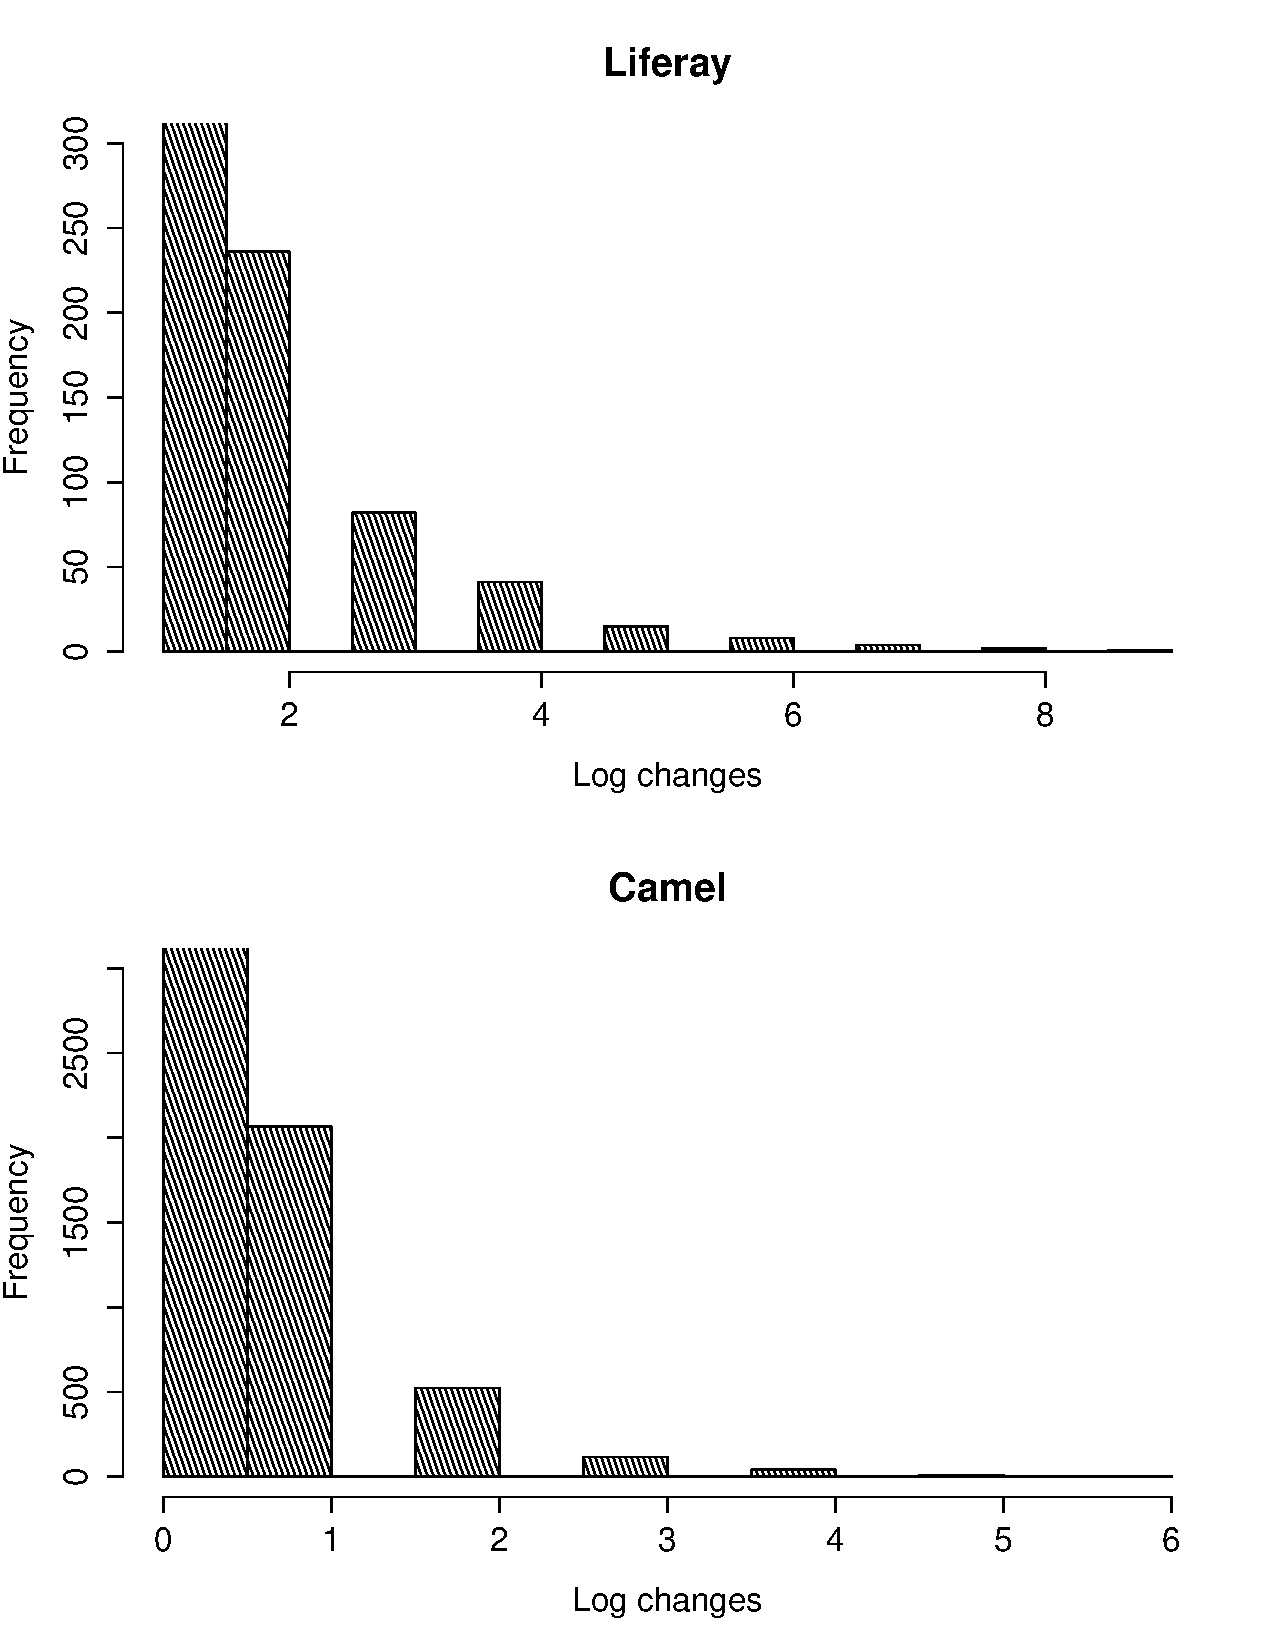
\includegraphics[width=0.7\linewidth]{RQ1_Liferay_Camel_Logchangefreq}
%	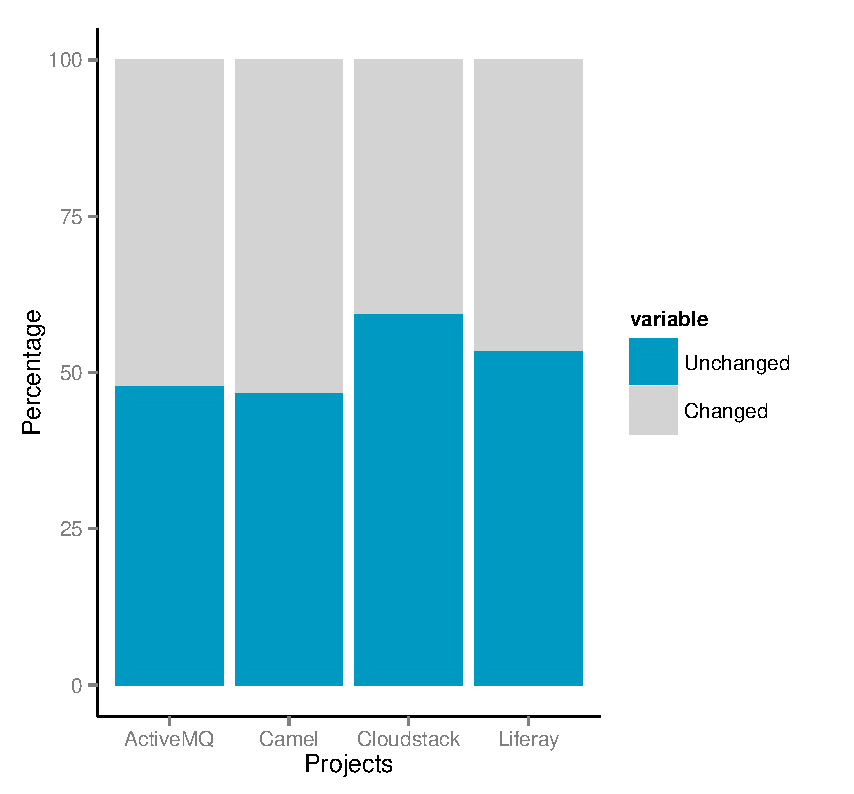
\includegraphics[width=0\linewidth]{Percentageofchanges}
%	\caption{Percentage of log changes in the studied applications.}
%	\label{fig:RQ1_Liferay_Camel_Logchangefreq}
%\end{figure}

\begin{figure}[tb]
	
	\centering
%	\captionsetup{justification=centre}
	
		\subfloat[Percentage of log changes]{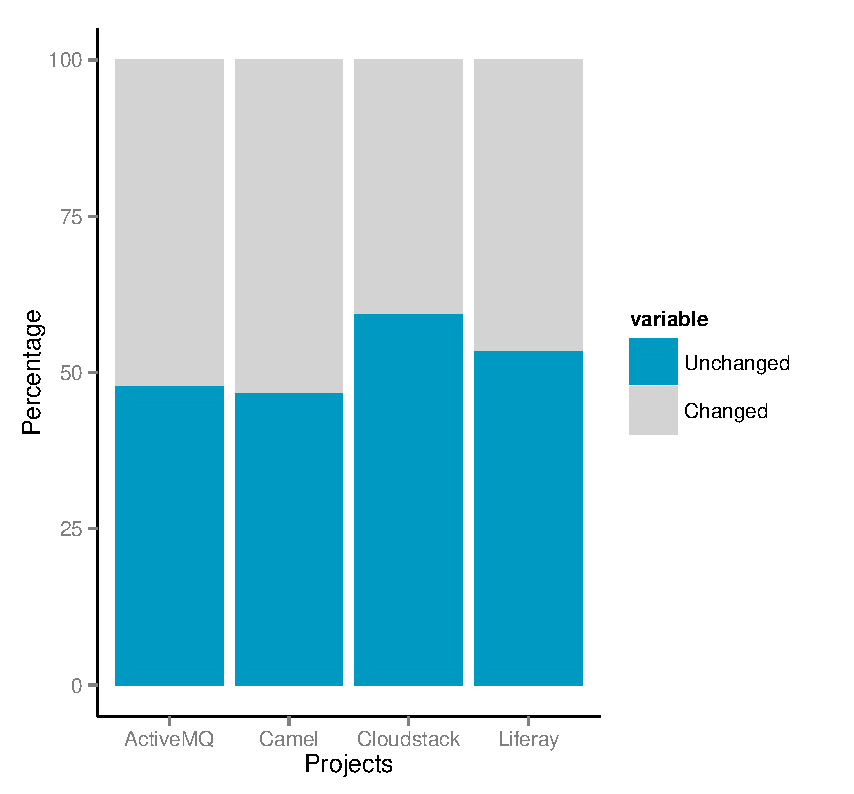
\includegraphics[width=0.5\linewidth]
			{Percentageofchanges}\label{fig:percentage} }

	\subfloat[Frequency of log changes]{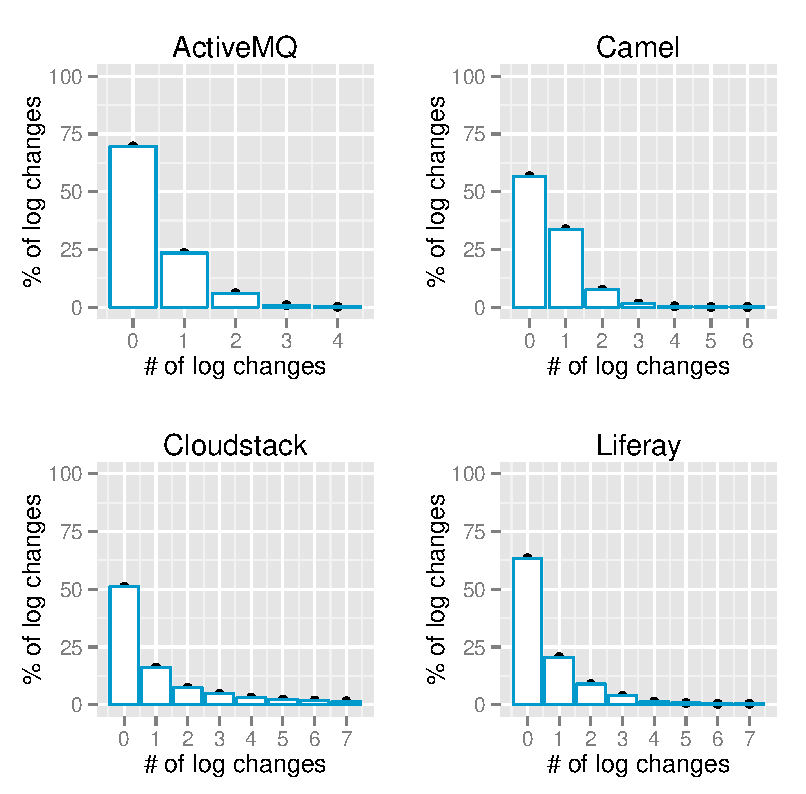
\includegraphics[width=1\linewidth]
		{frequencyofLogchanges}\label{fig:Feq} }
	
	%	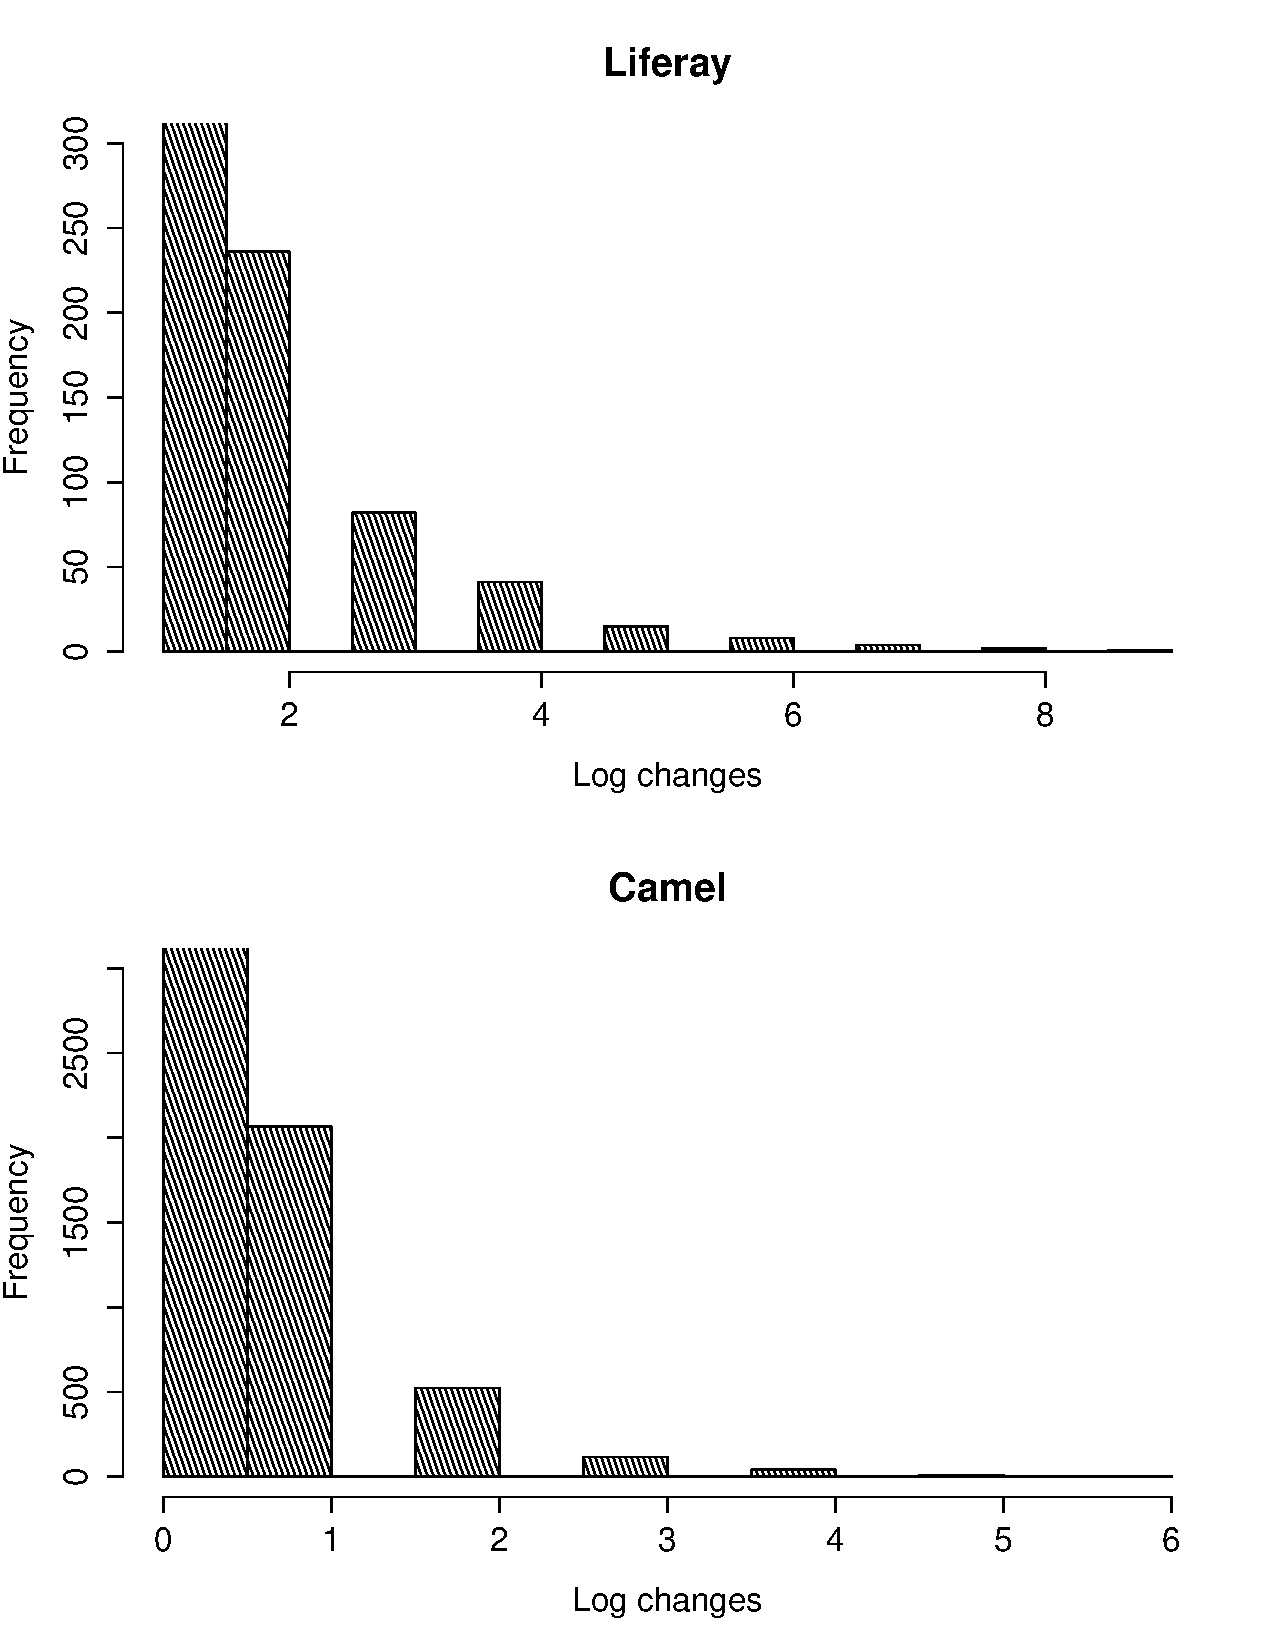
\includegraphics[width=0.7\linewidth]{RQ1_Liferay_Camel_Logchangefreq}
%	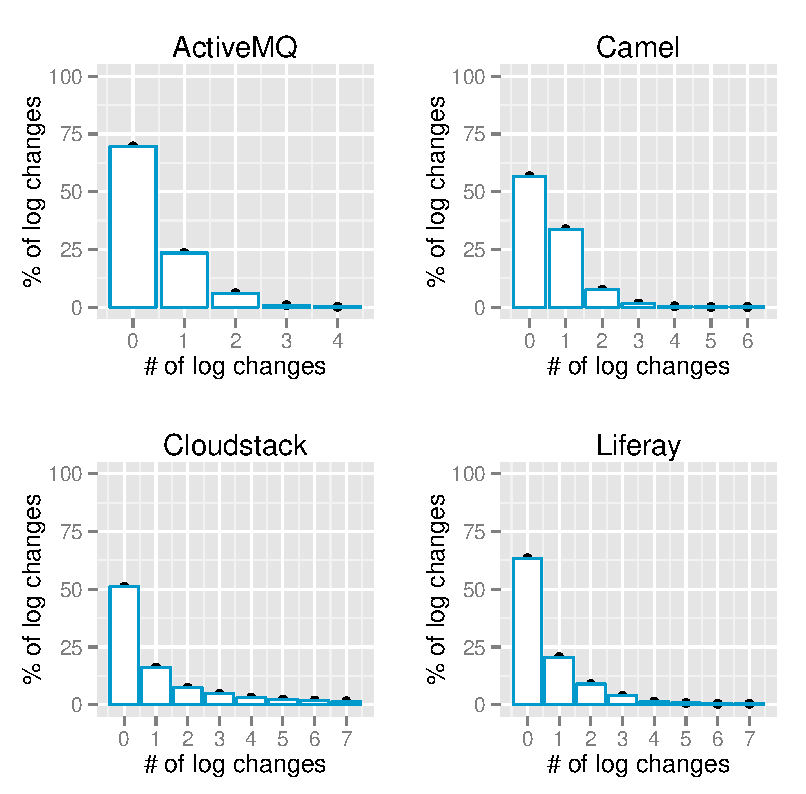
\includegraphics[width=0.9\linewidth]{frequencyofLogchanges}
	\caption{\protect \subref{fig:percentage}  shows the percentage of changed vs unchanged logs and \protect\subref{fig:Feq} shows the number of times logs are changed within the studied applications. } 
	\label{fig:frequencyofLogchanges}
\end{figure}



%To find how frequently logs change, we conduct a quantitative analysis on the studied systems. We use the tracked log data for each studied system as explained in Section~\ref{Methodology}. From each project, we select a random sample with 95\% confidence interval. We follow the same iterative process as in prior research~\cite{IanIcesm} to find how frequently logs change in our studied systems. 




\begin{figure}[tb]
	\centering
	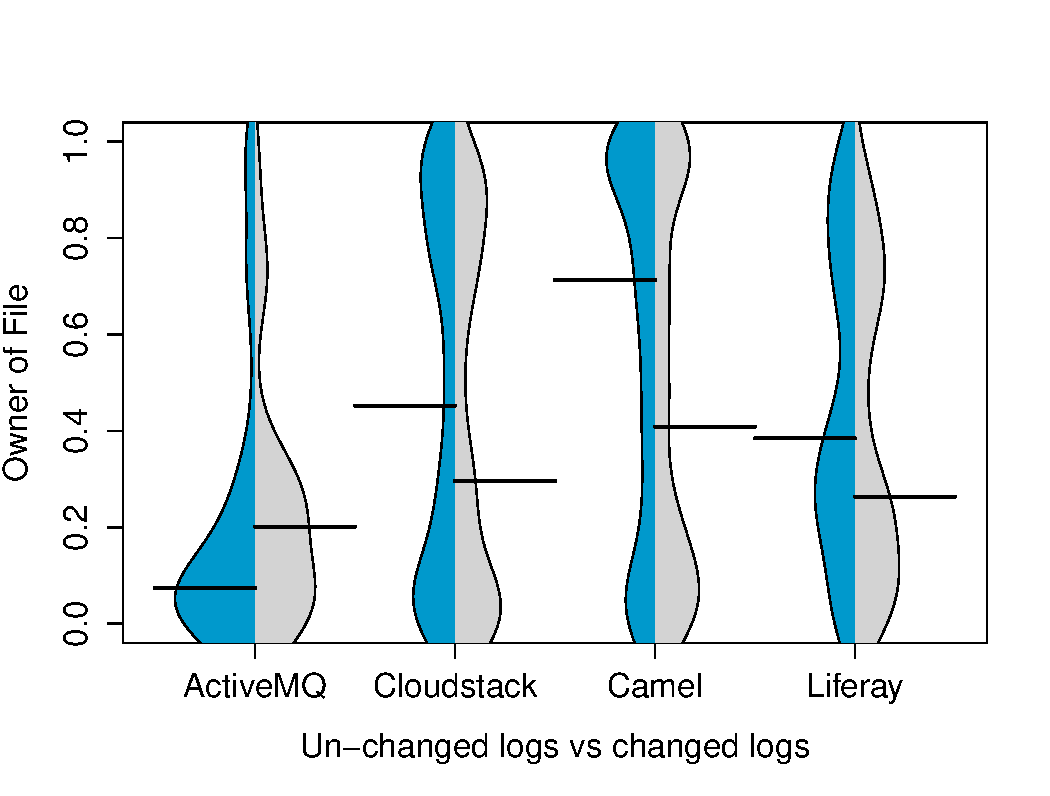
\includegraphics[width=1\linewidth]{ChangedvsUnchangedlogs}
	\caption{Distribution of logs which are changed vs un-changed against the ownership of the developer introducing the log}
	\label{fig:ChangedvsUnchangedlogs}
\end{figure}
\begin{figure}[tb]
	
	\centering
	%	\subfloat{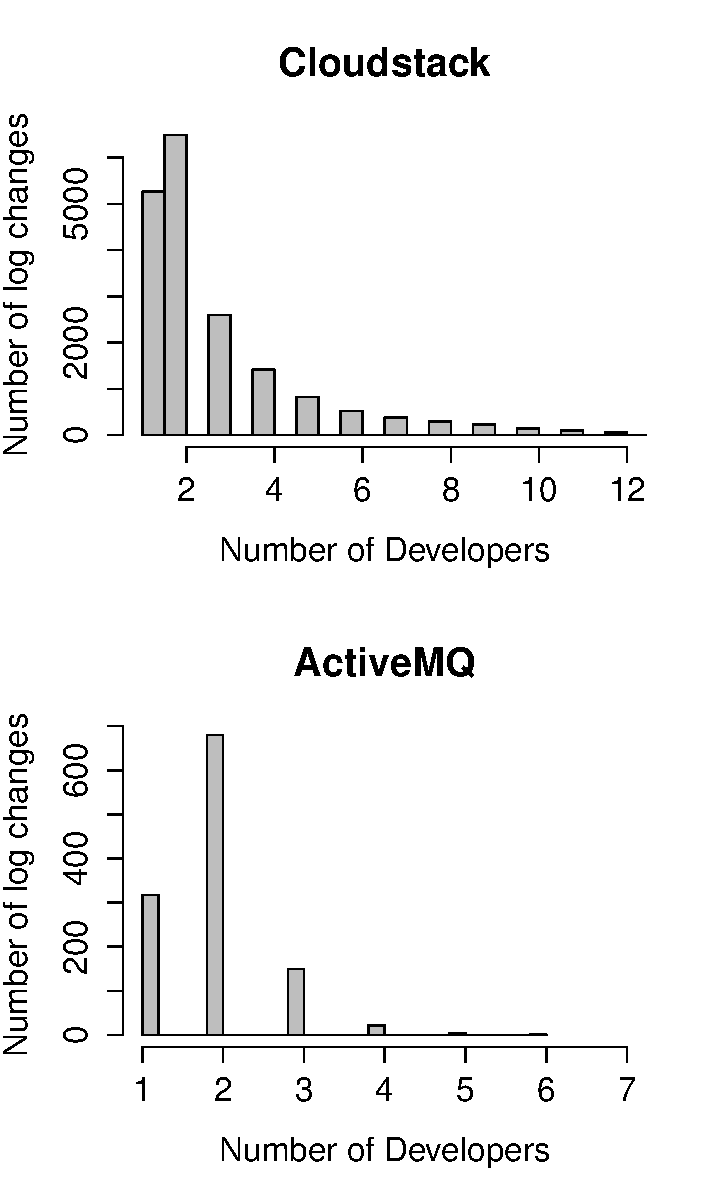
\includegraphics[width=0.5\linewidth]{CA_numberofDevelopers}\label{fig:f1}}
	%	\hfill
	\subfloat{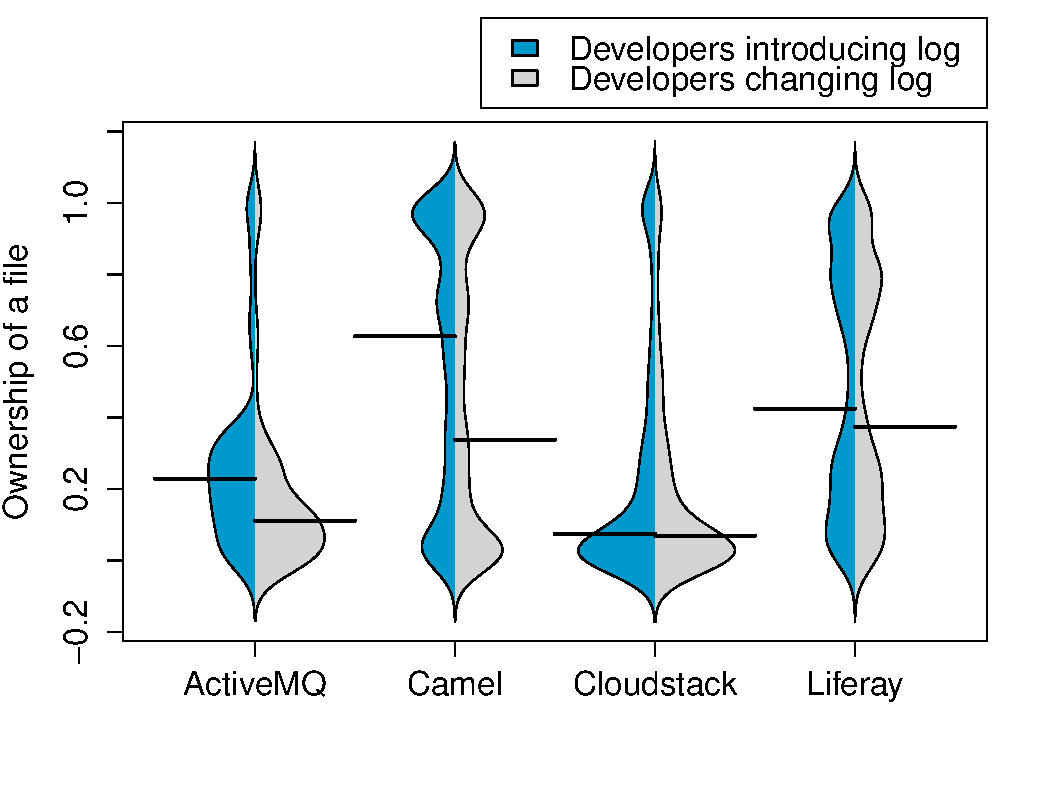
\includegraphics[width=1\linewidth]{ChangedvsChangesorNot}\label{fig:f2}}
	\caption{Distribution of file ownership against developers introducing the log vs developers changing the log.}
	\label{fig:ChangedvsChangesorNot}
\end{figure}



\begin{figure}[tb]
	
	\centering
	%	\subfloat{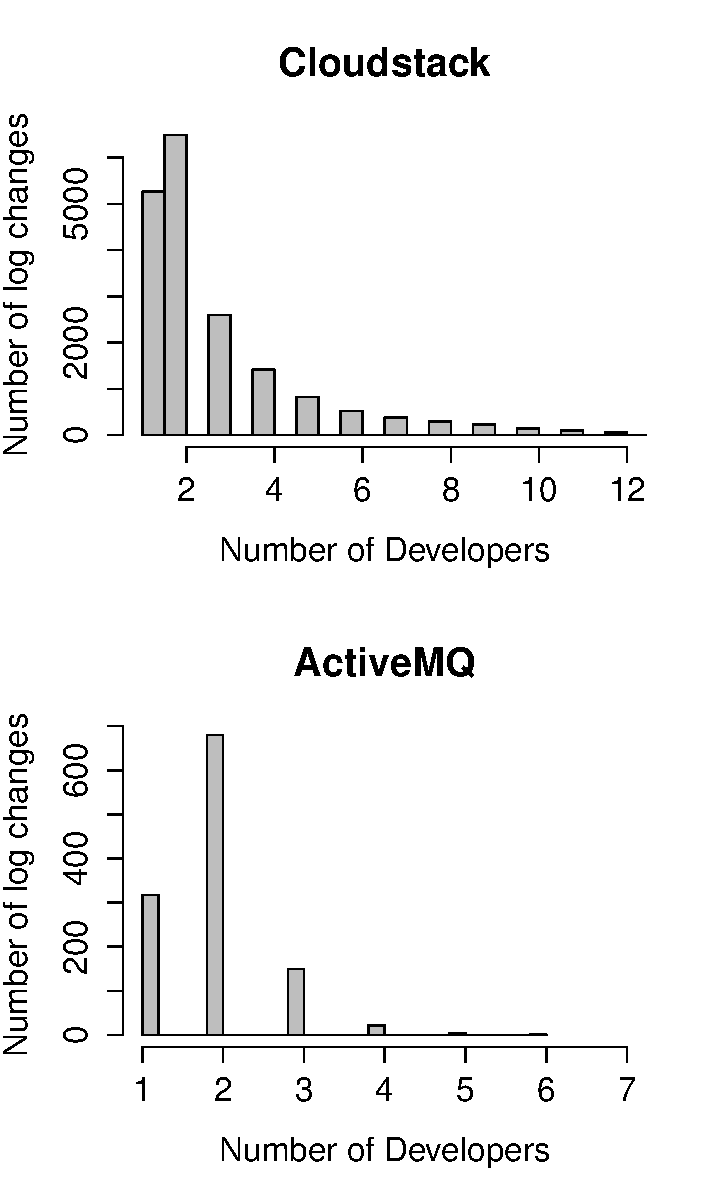
\includegraphics[width=0.5\linewidth]{CA_numberofDevelopers}\label{fig:f1}}
	%	\hfill
	\subfloat{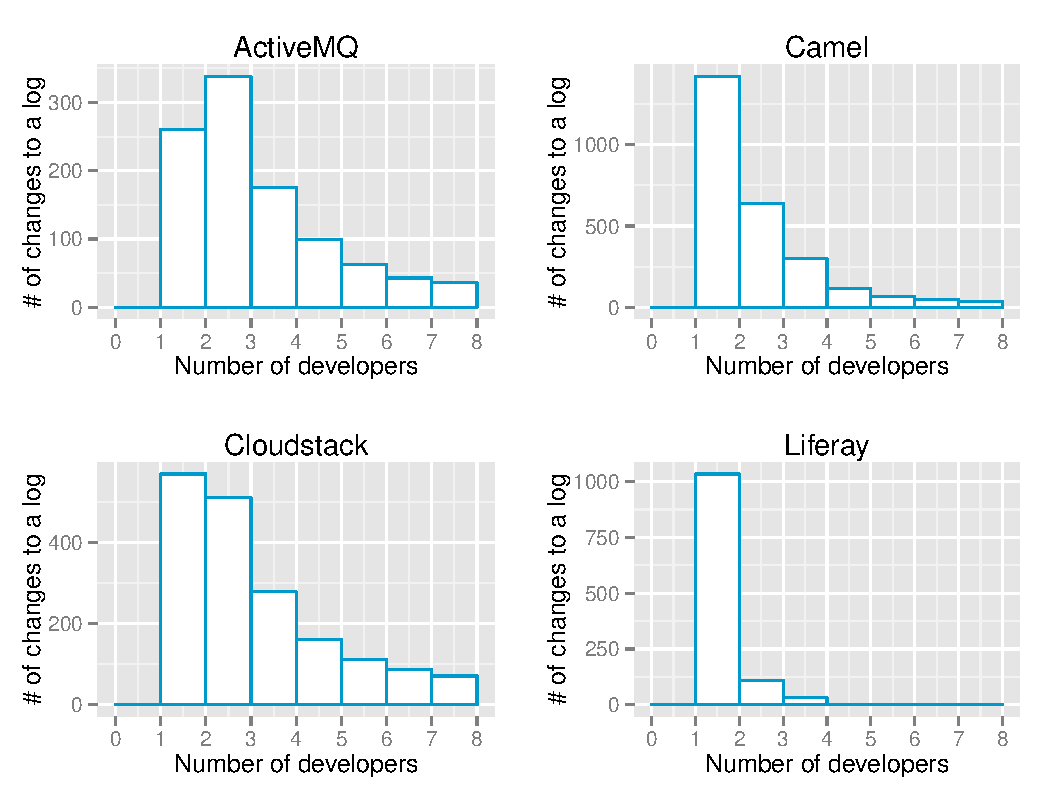
\includegraphics[width=1\linewidth]{NumberofDevelopers}\label{fig:f2}}
	\caption{Distribution of the number of developers responsible
		for changing a log.}
	\label{fig:NumberofDevelopers}
\end{figure}





\subsection{Results}

\subsubsection*{C.1. Change frequency}
\hypobox { Developers change 45\%-55\% of the logs across our studied applications. }
Figure~\ref{fig:frequencyofLogchanges} shows the percentage of changed logs in each of the studied applications. This shows that log change extensively throughout the lifetime of an application which can affect the log processing tools.
 
%as shown in Figure~\ref{fig:RQ1_Liferay_Camel_Logchangefreq}. 



%Based on frequency of changes, we categorize logs into 3 categories namely: a) Frequently Changed, b) Changed and c) Never Changed as shown in Table~\ref{tba:logchangeDistribution}. If a log is changed more than four times it is categorized as `Frequently Changed'. If it is changed 1 to 3 times it is categorized under `Changed' and if it did not change it is categorized under `Never Changed'. We select four as the threshold as we observe that majority of logs only have 1 to 2 changes as seen in Figure~\ref{fig:RQ1_Liferay_Camel_Logchangefreq}. We see that the majority of logs never change in Liferay and the majority of logs in ActiveMQ and CloudStack are changed atleast once. This may be because Liferay has fewer logs per source code file (i.e., lower log density) when compared to ActiveMQ and CloudStack as seen in Table~\ref{tba:overviewsystems}. 


\subsubsection*{C.2. Developer impact}
After identifying the frequency of changes within the studied applications, we find the number of the developers responsible for the log changes and also if they own the file which contains the log. We use the developer name available from the `git log' to count the number of developers who change a log. To decide whether a developer owns a file we calculate the ratio of number of lines written by him to the total lines of code using the `blame' command available in git. This is recursively done till the first commit of the file and the contribution of the developer at each commit is recorded.  We take the mean average of his contribution across all commits to obtain his ownership metric for the file. 



\hypobox{We see that logs which change are introduced by developers who have little ownership over the file.} 
Figure~\ref{fig:ChangedvsUnchangedlogs} shows that in Camel, Cloudstack and ActiveMQ, the logs which change are more likely to be introduced by developers who have less ownership on the files, than logs which are never changed. This suggests that logs can be introduced by non-owners of a file, which leads to logs being changed later. 

%We see that logs are changed by developers who have lesser ownership over the 
%file than the developers who introduce the log.

We see thats logs are also changed by developers who have lesser ownership than the ones introducing them. Figure~\ref{fig:ChangedvsChangesorNot} shows that in all the studied applications the logs are more likely to be changed by developers who have lesser ownership on the file than the developers who introduce the log. We find that in one of the studied applications the majority of logs are changed by two or more developers as seen in Figure~\ref{fig:NumberofDevelopers}. These results suggest that logs are readily changed by developers who access the file but do not have strong ownership characteristics.   



%These results suggest that logs are readily changed by developers who access the file but do not have strong ownership characteristics.

%Figure~\ref{fig:ChangedvsChangesorNot} shows that in all the studied


 

% which change are introduced by developers who have less ownership on files than the developers who introduce the log.
 
%  We also find that in one of the studied applications the majority of logs are changed by two or more developers as seen in Figure~\ref{fig:NumberofDevelopers}. 

% we see that in two of the studied systems, a single developer is responsible for majority of the log changes. 

%This suggests that logs can be 
% do not have strong ownership characteristics and can be changed by developers than one introducing the logs.

%\hypobox {45\%-55\% of the logs are changed atleast once in the studied applications. We find that over 51\% of the changes are made to the static content, variable content and log level. We also find that logs are changed by developers who have little ownership of the file and in two of the projects we find the majority of logs are changed by two or more developers.}

%When logs are changed, they can be changed in five possible ways namely:
%\begin{enumerate}
%	
%	\item { \textbf{Log relocation:} } The log is kept intact but moved to a different location in the file because of context changes (code around the log is changed).
%	
%	\item \textbf{Text change:} The text (i.e., static content) of log is changed. 
%	
%	\item\textbf{Variable change:} One or more variables in the log are changed (added, deleted or modified).
%	
%	\item \textbf{Change of log level:} The verbosity level of a log is changed.
%	
%	\item  \textbf{Text and variable change:} Both text and variables in the logs are changed. This is generally done when developers provide more context information, i.e, text and add/modify the relevant variables in a log.
%	
%\end{enumerate}
%
%%for several reasons. To understand the different types of log changes we perform a manual analysis on the changed logs. We select a random sample from each project such that the sample achieves 95\% confidence interval. After identifying the different types of log changes we automate the process of identification using our scripts. Figure~\ref{fig:Flowchart2} highlights the process of categorizing the log changes. For example,consider the logs shown below. 


%We see that there can be only four possible ways in which developers change logs namely:
%
%To automate the process of categorizing log changes into these categories, we first remove the logging method (i.e, LOG) and the log level (i.e, info) from the logs. We then compute the \textsl{Levenshtein ratio} between each term within the parentheses. In the example below we find that `+ Integer.toString(listenPort)' has \textsl{Levenshtein ratio} of 1, implying they are identical and the \textsl{Levenshtein ratio} between `starting HBase HsHA Thrift server on' and `starting HBase' is 0.56. This suggests there is some similarity between the two strings and the variable is constant which implies its a text change. (Figure~\ref{fig:Flowchart2} highlights the process of categorizing the log changes.
%
%\hypobox {+ LOG.info(``starting HBase HsHA Thrift server on " + Integer.toString(listenPort)); }
%
%\hypobox {- LOG.info(``starting HBase " + implType.simpleClassName() +`` server on " + Integer.toString(listenPort)); }



% ownership of file using the `blame' command available in git i.e.., if two developers are responsible for a file, but one has written 100 of the 150 lines of code, we calculate his 
%\begin{enumerate}
%	
%	\item { \textbf{Log relocation:} } The log is kept intact but moved to a different location in the file because of context changes (code around the log is changed).
%	
%	\item \textbf{Text change:} The text (i.e., static content) of log is changed. 
%	
%	\item\textbf{Variable change:} One or more variables in the log are changed (added, deleted or modified).
%	
%	\item \textbf{Change of log level:} The verbosity level of a log is changed.
%	
%	\item  \textbf{Text and variable change:} Both text and variables in the logs are changed. This is generally done when developers provide more context information, i.e, text and add/modify the relevant variables in a log.
%	
%\end{enumerate}
% 

%\noindent \textbf{Results}


%{\suhas{ I have question Can i tell here that in RQ2 we find log density to be imporatnt factor in stability of logs ?? }}

% are application layer software which  rely less on logs as they are middle-ware/application software, whereas ActiveMQ and CloudStack are service software.




%From manually analyzing the changed logs, we identify five types of log changes (i.e., changes to verbosity levels, log context, logged variables, both context and variable and relocation of log).  Table~\ref{tba:logtype} shows their distributions. When there is overlapping of the different types of log changes, we categorize them as newly added log and track changes made to it.

%	We find that about 3-11 \% of logs are changed frequently. This suggests that log processing tools which run on these systems need constant maintenance from developers

